\chapter{Data Analysis}

\section{Dredging activity}
This section describes the relevance of dredging to the sediment balance of the designated area, by an estimation of the dredging volumes through different data sources. It includes an analysis of the data gathered through AIS and extraction permits. 


\subsection{Vessel positioning information (AIS)}

Using MarineTraffic it was found that two dredgers are operating on the Paraná Guazú between Ibicuy and Brazo Largo: the Comercio Segundo and the E.M. Arroyo N1. The Comercio Segundo has a length of 30 m, a width of 7 m, a draft of 1.3 m, and an approximate cargo hold of 195 m\textsuperscript{3}. The E.M. Arroyo N1 has a length of 39 m, a width of 8 m, a draught of 2.8 m and an approximate cargo hold of 476 \,m\textsuperscript{3}. Using a sand to water ratio of 3:1 for the dredged slurry, the amount of sand dredged is 150 \,m\textsuperscript{3} and 360 \,m\textsuperscript{3} respectively per cargo. The tracks of the two vessels obtained from MarineTraffic are shown in Figures 5.1 and 5.2.

\begin{figure}[h!]
    \centering
    \begin{minipage}{0.48\textwidth}
        \centering
        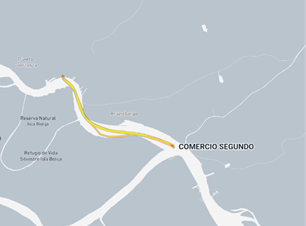
\includegraphics[width=\linewidth]{figures/ch5/Track_CS.png}
        \caption{Track of the \textit{Comercio Segundo}}
        \label{fig:track_cs}
    \end{minipage}\hfill
    \begin{minipage}{0.48\textwidth}
        \centering
        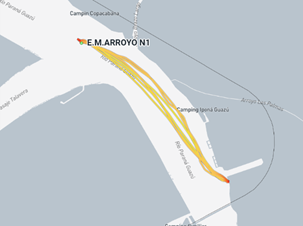
\includegraphics[width=\linewidth]{figures/ch5/Track_EM.png}
        \caption{Track of the \textit{E.M. Arroyo N1}}
        \label{fig:track_em}
    \end{minipage}
\end{figure}

The AIS data for these two vessels is obtained from MyShipTracking, which is used to determine the location of the dredging and the average number of trips. The dredging location of the two vessels is shown in Figure 5.3. It can be seen that both dredgers dredge in the same area. This can be explained by the bathymetry shown in Figure 5.4, which shows a reduced depth near the junction of the two navigable channels. At this location the flow velocity is lower, causing sediment to settle and thus creating a sandbar. From the AIS data it can be concluded that both dredgers make three trips per day.

\begin{figure}[h!]
    \centering
    \begin{minipage}{0.48\textwidth}
        \centering
        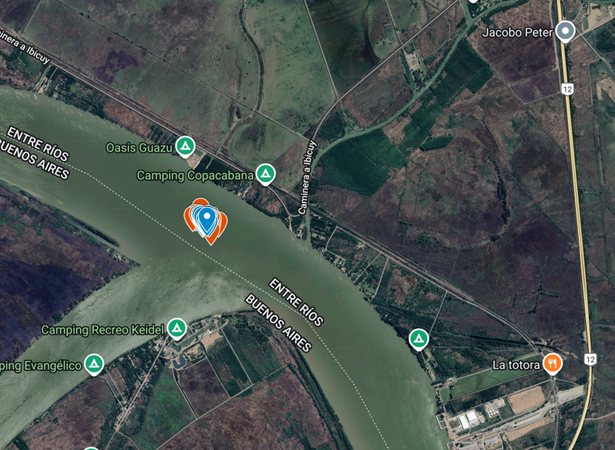
\includegraphics[width=\linewidth]{figures/ch5/Dredging_coordinates.png}
        \caption{Dredging location}
        \label{fig:dredging_coordinates}
    \end{minipage}\hfill
    \begin{minipage}{0.48\textwidth}
        \centering
        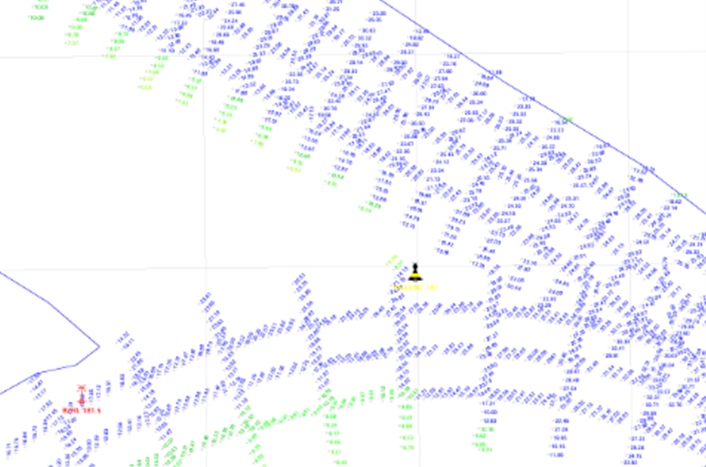
\includegraphics[width=\linewidth]{figures/ch5/Bathymetry.png}
        \caption{Bathymetry}
        \label{fig:bathymetry}
    \end{minipage}
\end{figure}

In the Rio Talabera, a side branch connecting to the Paraná Guazú, a third dredger is extracting sand. The Altair is dredger with a length of 66 m, a width of 11 m, a draught of 1.5 m and a approximate cargo hold of 750 \,m\textsuperscript{3}. Using the same sand to water ratio of 3:1 this gives 560 \,m\textsuperscript{3} of sand per cargo. Using MarineTraffic it was found that the Altair has an average 3 trips per day. Figure 5.5 shows the track of the Altair and the location at which it stops to extract sand. 

\begin{figure}[H]
    \centering
    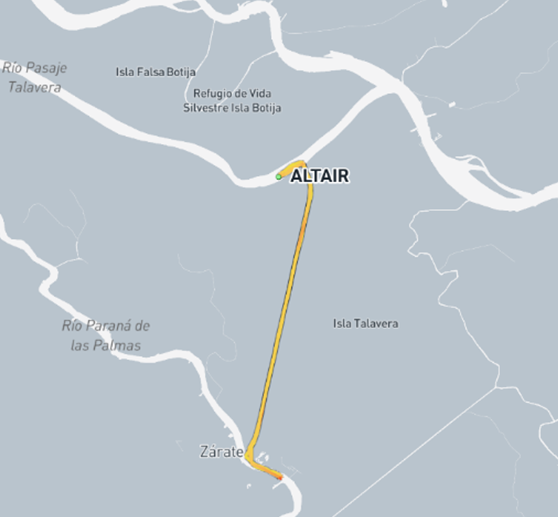
\includegraphics[width=0.5\linewidth]{figures/ch5/Track_Altair.png}
    \caption{Track of the Altair}
    \label{fig:placeholder}
\end{figure}

For all three vessels, the estimated volume of sand extracted per month is displayed in table 5.1
\begin{table}[h!]
\centering
\begin{tabular}{lrrrr}
\hline
\textbf{Vessel} & \textbf{Cargo hold} & \textbf{Sand volume [\,m\textsuperscript{3}]} & \textbf{Trips per day} & \textbf{Volume per month [\,m\textsuperscript{3}]} \\
\hline
Comercio Segundo & 195 & 150 & 3 & 9000 \\
E.M. Arroyo N1 & 476 & 360 & 3 & 21600 \\
Altair & 750 & 560 & 3 & 33600 \\
\hline
\end{tabular}
\caption{Sand transport details per vessel.}
\label{tab:sand_volume}
\end{table}


\subsection{Extraction permits}
A total of 33 permits were collected for the Paraná Guazú and 43 for the Ibicuy. On the Paraná Guazú, four permits were issued for channel maintenance, while the remainder concerned sand extraction. For the Ibicuy, all permits were related to extraction activities. The analysis shows that the requested volumes in the Ibicuy are considerably larger than those in the Paraná Guazú, even though the section of the Ibicuy considered here is much shorter in length.

It is important to note that the end dates of contracts are unknown. While the requests specify monthly dredging quantities, they do not indicate the duration of the works. As a result, a detailed quantitative assessment cannot be made. For the present analysis, all requests with fixed monthly volumes are assumed to extend over 12 months, allowing for a comparison between the two river sections, as shown in Figure \ref{fig:yearly dredging volumes}. The second assumption is to record a single value for the requested volume, when information about monthly or yearly occurrence is lacking.

\begin{figure}[H]
    \centering
    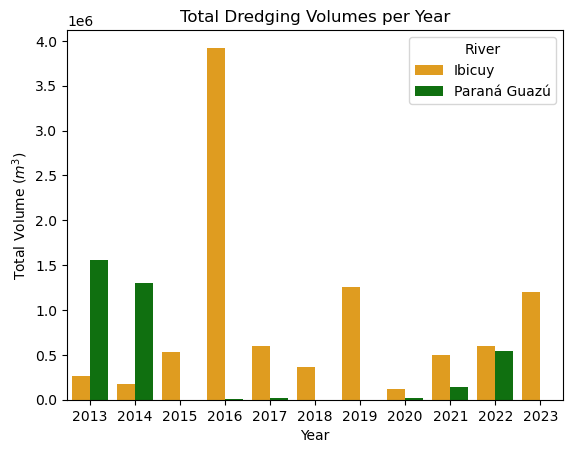
\includegraphics[width=0.50\linewidth]{figures/ch2/Dredging volumes permits.png}
    \caption{Yearly dredging volumes}
    \label{fig:yearly dredging volumes}
\end{figure}

\subsection{Estimated sand extraction}
This section draws a conclusion on the sand extraction volumes, such that an estimate is found to apply in the sediment balance. The following uncertainties were considered in determining a representative value:

\begin{itemize}
    \item Not every vessel in the area is equipped with an AIS transponder, meaning that possibly not all active vessels were identified
    \item No historical AIS data was available, such that the data was registered for only a short period of time 
    \item The extraction permits do not mention the duration of the contract
\end{itemize}

However, a rough estimate can be found by calculating the mean annual volume for the total system of interest (i.e., Ibicuy and Paraná Guazú). To make a comparison with the monthly values in Table \ref{tab:sand_volume}, this yearly value is reduced to a monthly value by dividing by 12 months. The former approach yields the following value for dredged sand volumes:

\begin{equation}
    V_{sand,yearly} = 1193923 ~m^3
\end{equation}
\begin{equation}
    V_{sand,monthly} = \frac{V_{sand,yearly}}{12} \approx 100000 ~m^3 
\end{equation}


\section{Hydrodynamic data}
nog introductie toevoegen

\\ \textbf{Tidal forcing}
\\The tidal wave of the Atlantic Ocean influences the hydrodynamics of the lower Paraná delta. As the tidal wave enters the delta ta Río de la Plata, the tide is damped and phased by friction, channel geometry and branching, resulting in a reduced amplitude and an increased in phase delay. Under normal conditions, the influence of the tide on the Paraná River reaches the city of Villa Constitución, which is located 220 km upstream of the river mouth. For storm conditions, the tide can reach the city of Rosario \autocite{balayCAUSESPERIODICITYLARGE}. In order to determine the influence of the tide at Brazo Largo, a reference water level at San Fernando is considered. It is assumed that at San Fernando no tidal damping has occurred, therefore the tidal amplitude at Brazo Largo can be determined using the following relation:
\[
A_{\text{Location}} = \alpha \cdot A_{\text{SanFernando}}
\]
The damping coefficient ($\alpha$) and the tidal delay with respect to San Fernando have been determined by Brok (2022). For Brazo Largo, a damping coefficient of 0.3 and tidal delay of 4 hours were found. These values will be used as reference values when isolating the tide at Brazo Largo. The tidal signal is isolated using hourly water level data for a period of more than 2 years from both Brazo Largo and San Fernando. Table 5.2 shows the tidal constituents  considered and their period.

\begin{table}[h!]
\centering
\caption{Tidal constituents used to reconstruct the tide
\autocite{BRON}.}
\label{tab:constituents}
\begin{tabular}{lccc}
\hline
\textbf{Tidal constituent} & \textbf{Name} & \textbf{Period [h]} \\
\hline
\multicolumn{3}{l}{\textit{Semi-diurnal}} \\
\hspace{1em}Principal lunar & M2 & 12.4206\\
\hspace{1em}Principal solar & S2 & 12.0000 \\
\hspace{1em}Lunar elliptical & N2 & 12.6583\\
\hline
\multicolumn{3}{l}{\textit{Diurnal}} \\
\hspace{1em}Lunar-solar declinational & K1 & 23.9345  \\
\hspace{1em}Principal lunar & O1 & 25.8193  \\
\hline
\multicolumn{3}{l}{\textit{Shallow water constituents}} \\
\hspace{1em}Overtide of M2 (quarter-diurnal) & M4 & 6.2103  \\
\hline
\end{tabular}
\end{table}

- uitleg hoe het getijde bepaald is

Figure 5.7 shows the water level time series for a period of 7 days compared to the calculated tidal signal at Brazo Largo. From this figure, it can be seen that the measured water level follows the same tidal oscillations. However, the tide does not explain all the variability of the water level; the measured water level also shows large variability caused by discharge and wind. 

\begin{figure}[H]
    \centering
    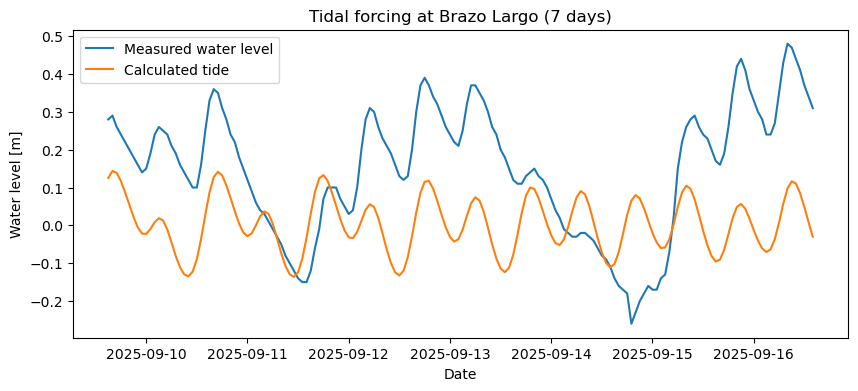
\includegraphics[width=1\linewidth]{figures/ch5/Tide_Brazo_largo.png}
    \caption{Reconstructed tide at Brazo Largo}
    \label{fig:placeholder}
\end{figure}



\begin{table}[h!]
\centering
\caption{Amplitude and phase comparison}
\begin{tabular}{lcccccc}
\hline
Constituent & $A_{\text{SF}}$ & $A_{\text{BL}}$ & $\alpha$ & tide delay [hr] & $\phi_{\text{SF}}$ [$^\circ$] & $\phi_{\text{BL}}$ [$^\circ$] \\
\hline
M2 & 0.253 & 0.058 & 0.230 & 4.450 & -0.465 & 1.786 \\
S2 & 0.041 & 0.010 & 0.239 & 5.055 & -2.526 & 0.121 \\
N2 & 0.094 & 0.022 & 0.238 & 4.316 & -0.546 & 1.596 \\
K1 & 0.119 & 0.037 & 0.313 & 5.181 & -2.543 & -1.183 \\
O1 & 0.187 & 0.061 & 0.328 & 5.517 & 2.694 & -2.247 \\
M4 & 0.030 & 0.006 & 0.189 & -1.495 & -2.608 & 2.162 \\
\hline
\end{tabular}
\end{table}



\\- Waterlevel at Brazo Largo
    (misschien het getijde meenemen?)
\\ - Getijde rond Brazo Largo is berekend aan de hand van waterlevel rond San Fernando. Vergelijk de constituents met die van  het rapport en trek conclusie over invloed getijde.

\textbf{Fluvial forcing}

The relationship between fluvial discharge and water level at Brazo Largo was initially assumed to follow a power-law ($h = a \cdot Q^b$), but this yielded a weak correlation with an $R^2$ of 0.261. A linear fit, however, produced a slightly better result, showing a positive trend with an $R^2$ of 0.444 (Figure \ref{fig:waterleveldischarge}).

In contrast, the El Colorado and Túnel Subfluvial stations exhibit a clear power-law dependence. Power-law fits for these stations resulted in higher $R^2$-values of 0.962 and 0.712, respectively, with the El Colorado plot shown in Figure \ref{fig:waterleveldischarge}. Overall, these results suggest that the strength of the water level–discharge relationship decreases as the river flows downstream.

\begin{figure}[h!]
    \centering
    % First subfigure
    \begin{subfigure}[b]{0.48\linewidth}
        \centering
        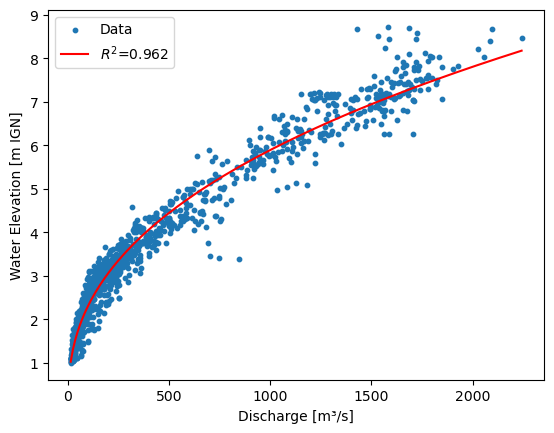
\includegraphics[width=\linewidth]{figures/ch5/wl discharge El Colorado.png}
        \label{fig:water level discharge Colorado}
    \end{subfigure}
    \hfill
    % Second subfigure
    \begin{subfigure}[b]{0.48\linewidth}
        \centering
        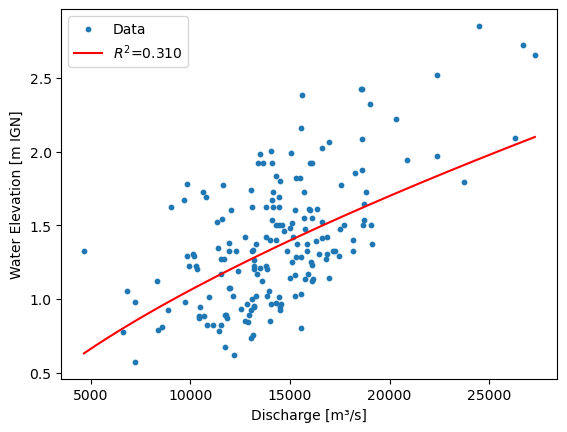
\includegraphics[width=\linewidth]{figures/ch5/wl discharge Brazo Largo.png}
        \label{fig:water level discharge Brazo Largo}
    \end{subfigure}
    \caption{Water elevation - discharge relationship for two measurement stations}
    \label{fig:waterleveldischarge}
\end{figure}



The Paraná Guazu is influenced by both tidal and fluvial controls.
    

- Flow partitioning:
    Gebruik debiet van parana en parana Guazu (zie plot in VScode)
    Gebruik veldwerk metingen om bijdrage rio Ibicuy en rio Talabera te bepalen


\section{Sediment transport}
From the Brazo Largo measurements, an analysis can be done on the relationship between sediment concentrations and the discharge of the river. Again, a distinction can be made between fine and course sediments. Overall, a power-law fit seems a good approach to model the relation, as show. The fine sediment concentration is generally higher than the course sediment concentration. In addition, the course se



- Bepaal fine sediment-discharge relation bij El Colorado. Reken hiermee door voor het fine sediment concentration bij Brazo Largo

- Bepaal fine sediment concentration op basis van de suspended sediment samples.

- Coarse sediment concentration wordt bepaald met de Engelund-Hansen formule

- Vergelijk dit met de bedload metingen van het veldwerk

- Set up a sediment balance for the area of interest.


- Sediment transport caused by tidal assymetry.
% \section{Water Quality and Bioorganism Activity?}

